\xchapter{Revis\~{a}o Bibliogr\'{a}fica}  {} \label{revisao}
\section{Considerações Iniciais}

Em Aprendizado de Máquina não-supervisionado, técnicas de agrupamento visam encontrar padrões e extrair estruturas sobre conjuntos de dados sem qualquer informação à priori, utilizando apenas os valores dos atributos de cada instância. A etapa mais importante dos algoritmos de agrupamento é a utilização de medidas que permitem calcular a similaridade ou a distância entre os dados. De maneira geral, esses algoritmos buscam manter em um mesmo grupo dados mais similares. Quando dados analisados são organizados como Séries Temporais, a complexidade no cálculo da similaridade/distância aumenta devido à presença de uma dependência temporal entre as observações \cite{Aghabozorgi2015, zhang2011}. 
 
A dependência temporal entre observações de séries temporais é determinada pela presença de diferentes componentes como, por exemplo, a estocasticidade e o determinismo. Conforme discutido em \citeonline{Araujo2013, Araujo2015}, analisar séries temporais utilizando um único modelo pode produzir erros, uma vez que o componente estocástico é desconsiderado por técnicas de modelagem determinística e modelos estocásticos tendem a não analisar importantes informações no espaço topológico como atratores e repulsores. Este projeto de mestrado estende a abordagem apresentada em \cite{Araujo2013, Araujo2015} para permitir que o agrupamento de dados seja realizado considerando, de maneira individual, as influências estocásticas e determinísticas das séries.

Este capítulo apresenta uma discussão geral sobre os principais temas abordados neste projeto. Inicialmente, serão apresentados conceitos básicos sobre análise de séries temporais. Em seguida, a técnica de decomposição de série temporal em componentes estocásticos e determinísticos, que será utilizada neste projeto, é discutida em detalhes. Por fim, conceitos de agrupamento de séries temporais são apresentados, fornecendo detalhes sobre as principais medidas de similaridade/determinismo utilizadas na literatura.

\section{S\'{e}ries Temporais}

Uma série temporal pode ser definida como uma sequência de observações coletados ao longo do tempo $X_{t}={x_{0},x_{1},x_{2},...,x_{t}}$ \cite{box2015,Chouakria2007,morettin2006}. Uma série temporal univariada é composta por valores escalares, enquanto que as multivariadas possem múltiplas dimensões dentro da mesma faixa de tempo \cite{box2015,Chouakria2007}. Séries temporais podem ser caracterizadas, ainda, pelo intervalo entre coleta de observações que pode ser discreta ou contínua. Quando este intervalo é definido em tempos fixos, tem-se uma série discreta. Caso contrário, a série é dita ser contínua \cite{box2015, morettin2006}.  

Além disso, é importante enfatizar que séries temporais podem ser classificadas de acordo com a linearidade, estacionariedade e a estocasticidade de suas observações. Uma  série é dita linear quando os valores de suas obervações são determinados por uma uma combinação linear de ocorrências e ruídos passados. Quando a série é formada por sistemas cuja regra geradora são compostas por funções não-lineares, a série é dita ser não-linear \cite{box2015}.

As séries estacionárias assumem que as obervações estão em equilíbrio estatístico com propriedades que não mudam ao longo do tempo. Em séries estacionárias, sua média e variância são constantes. Quando essas propriedades mudam ao longo do tempo, a série é dita ser não-estacionária e, possivelmente, apresenta um comportamento de tendência   \cite{box2015,cryer2008}.

Por fim, séries podem ser classificadas em estocástica ou determinística. Quando apresentam um comportamento determinístico, o valor de suas observações possuem uma estrita relação de dependência com observações passadas. Séries estocásticas são constituídas por observações e relações aleatórias que seguem funções de densidade de probabilidade e podem se modificar ao longo do tempo, dificultando a modelagem de seus eventos \cite{box2015, morettin2006}.

Segundo \citeonline{box2015}, observações de séries temporais podem ser escritas na forma $x_{t}=T_{t}+S_{t}+ \varepsilon_{t}$, onde $T_{t}$ representa a tendência, $S_{t}$ representa a sazonalidade e $\varepsilon_{t} $ representa os componentes aleatórios. Se o componente $T$ está presente, a série é dita não-estacionária. Como pode ser visto nesta formulação, a sazonalidade é referenciada como sendo um componente determinístico e $\varepsilon$ como sendo um componente estocástico. Na Figura \ref{seri} são mostradas três séries influenciadas por tais componentes. 

\begin{figure}[!ht]
\begin{center}
  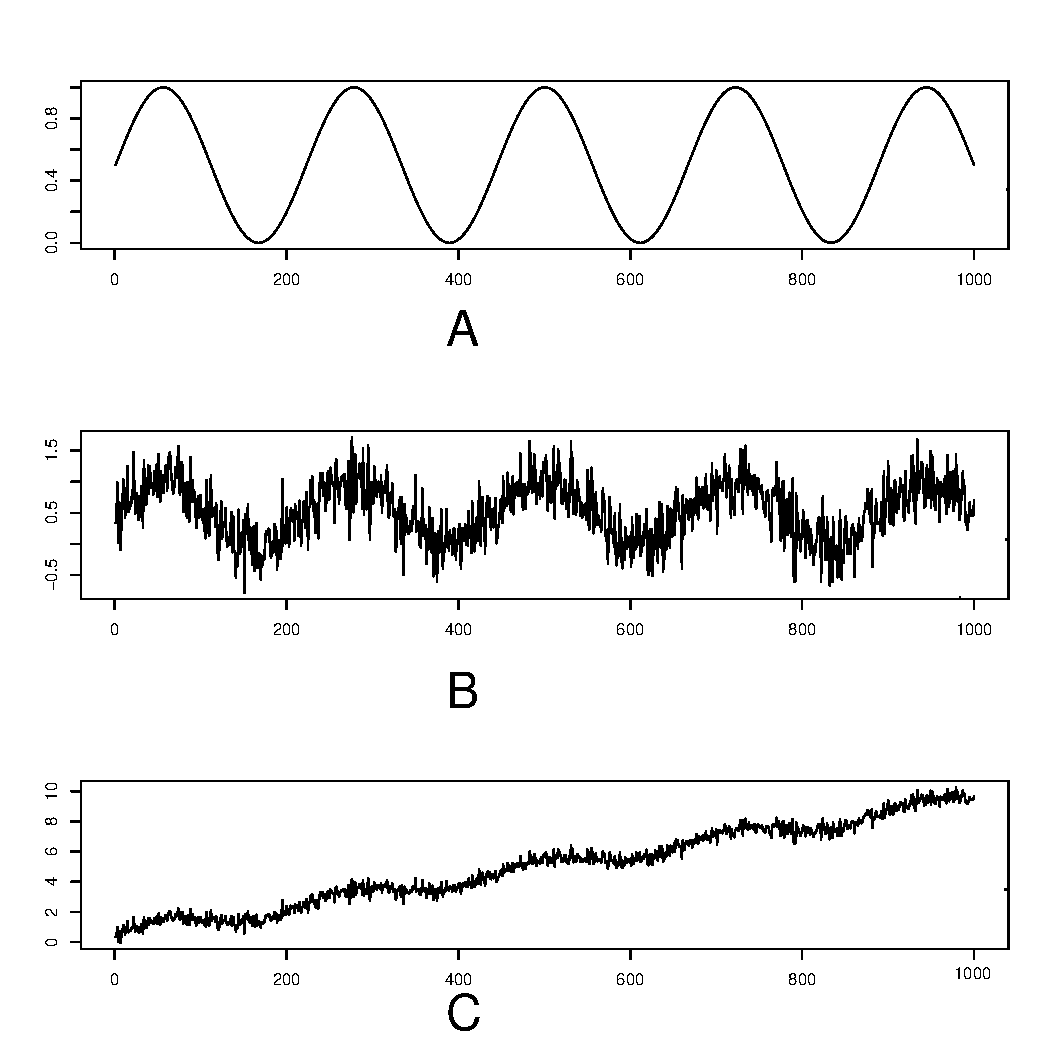
\includegraphics[scale=0.5]{seri7.pdf}
\caption{Séries temporais: (A) Sazonalidade. (B) Sazonalidade+ Componente aleatório. (C) Sazonalidade + Componente aleatório + Tendência.}
\label{seri}
\end{center}
\end{figure}

%% O uso de séries temporais pode ser classificado de acordo com  sua aplicação: Predição, Estimação de funções de transferência, análise de efeitos na intervenção de eventos e sistemas de controle. \cite{wu et al 2010}

Neste projeto de mestrado, serão consideradas séries univariadas, cujas observações são definidas por um ruído aditivo gerado a partir da combinação entre componentes estocásticos ($\varepsilon$) e determinísticos ($S$ e $T$).

\section{Análise de Séries Temporais}

O processo de análise de séries temporais tem como objetivo estimar uma regra (ou função geradora) para modelar o comportamento de suas observações, visando estudar e/ou predizer o comportamento de sistemas reais \cite{box2015, shum2006}. 

%A modelagem de sSão utilizados os sistemas dinâmicos e os modelos estatísticos para modelar séries. Os \textbf{sistemas dinâmicos} servem para a modelagem de séries determinísticas e os \textbf{modelos estatísticos} consideram eventos aleatórios, assim são utilizados para modelar séries estocásticas, incluindo as séries temporais lineares estacionárias e não-estacionárias \cite{alligood1997,box2015}.

No entanto, como já citado anteriormente, os sistemas do mundo real produzem séries com uma mistura de comportamentos estocásticos e determinísticos \cite{han2009}. Nesse caso, é importante utilizar modelos que analisem de forma individual a influência de cada comportamento. 

Para alcançar esse objetivo, \citeonline{Araujo2013,Araujo2015} desenvolveram uma técnica que permite decompor séries temporais em componentes estocásticos e determinísticos.

Essa técnica foi baseada no método de \ac{EMD} (\emph{Empirical Mode Decomposition}) \cite{Huang1998}. De maneira geral, \ac{EMD} decompõe uma série temporal em um conjunto de monocomponentes chamados IMF's (\emph{Intrinsic Mode Function}). Considerando que os IMF's revelam diferentes informações implícitas presente nos dados, \citeonline {Araujo2013, Araujo2015} utilizaram diferentes abordagens para medir o nível de determinismo presente em cada IMF e, consequentemente, combinar IMFs gerando os componentes estocásticos e determinísticos. 

No contexto deste trabalho de mestrado, essa técnica de decomposição permitirá separar séries temporais de acordo com suas influências estocásticas e determinísticas. Em seguida, essas influências serão individualmente analisadas pelos algoritmos de agrupamento, visando particionar o conjunto de séries temporais com maior acurácia. Na próxima seção, serão discutidos os principais conceitos de agrupamento de séries temporais.


\section{Agrupamento de Séries Temporais}

%Em \ac{AM} são utilizados algoritmos específicos para a mineração de dados com o intuito de descobrir conhecimento em conjunto de dados \cite{Mitchell:1997:ML:541177}. Segundo \citeonline{Mitchell:1997:ML:541177}, ``um programa de computador aprende com a experiência E, uma classe de tarefas T e a medida de desempenho P, seu desempenho em tarefas em T, medido por P, melhora com a experiência E \footnote[1]{A computer program is said to learn from experience E with respect to some class of tasks T and performance measure P, if its performance at tasks in T, as measured by P, improves with experience E.}. "
 
 %Os algoritmos que englobam as tarefas de \ac{AM}, são divididos em aprendizado supervisionado e aprendizado não-supervisionado. O aprendizado supervisionado conhece a saída dos dados, utilizando-a como rótulo. O aprendizado não-supervisionado não utiliza rótulo, sua função é descrever e/ou explorar o conjunto de dados sem treinamento prévio. O agrupamento de dados é uma técnica do tipo não supervisionada, a qual gera grupos(\textit{clusters}, conforme a proximidade dos dados. A proximidade dos dados é calculada com medidas de similaridade/distância \cite{faceli2011inteligencia, Mitchell:1997:ML:541177,xu2009}.
 
O agrupamento de séries temporais busca encontrar padrões em dados, cujas observações são caracterizadas por uma dependência temporal, \emph{i.e}, a ordem de coleta das observações é importante para a análise. O agrupamento de séries temporais é um tema relevante e tem sido utilizado em diversas pesquisas tais como, Medicina \cite{blei2015}, Aviação \cite{Ayhan2016} , Genética \cite{izakian}, Financeira \cite{durante} e detecção de anomalias \cite{Esling2012,Aghabozorgi2015}.


Segundo \citeonline{Aghabozorgi2015}, o agrupamento de séries temporais pode ser dividido em três categorias: i) agrupamento sobre diferentes séries temporais; ii) agrupamento de janelas de observações visando encontrar padrões de comportamento em uma mesma série temporal; e iii) agrupamento de ponto temporal que visa encontrar, em uma mesma série temporal, observações semelhantes. As principal diferença entre a categoria (ii) e (iii) é que a última não precisa definir uma janela fixa de observações.

De acordo \citeonline{bagnall2005}, o agrupamento de séries temporais é realizado considerando $3$ diferentes objetivos: i) tempo; ii) formato; e iii) mudança. Com relação ao tempo, algoritmos de agrupamento analisam séries calculando a similaridade entre observações coletadas em um mesmo instante de tempo. Com relação à forma, algoritmos visam agrupar séries temporais com comportamento geral semelhante, ou seja, com padrões recorrentes, visando encontrar um melhor alinhamento nos dados. Por fim, existem algoritmos cujo objetivo é avaliar a similaridade entre séries extraindo novas características como, por exemplo, a presença de tendência ou componentes implícitos. Neste caso, os algoritmos de mudança são geralmente executados sobre as características extraídas e não diretamente sobre as séries.

Ainda segundo \citeonline{Liao2005}, séries temporais podem ser agrupadas considerando três abordagens: i) aplicação de agrupamento sobre dados brutos, ou seja, sem qualquer transformação nas observações coletadas; ii) extração de características e aplicação de algoritmos de agrupamento convencionais sobre as características; e iii) modelagem de cada série e aplicação do agrupamento sobre cada modelo obtido.

Neste projeto de mestrado, será estudada a categoria de agrupamento aplicada sobre bases de dados compostas por diferentes séries temporais. Com relação ao objetivo, este projeto visa permitir que agrupamentos no tempo, no formato e na mudança sejam realizados com maior acurácia ao analisar, individualmente, os componentes estocásticos e determinísticos de cada série.

Por fim, espera-se que essa análise individual dos componentes permita melhorar o resultado de métodos de agrupamento que executam diretamente sobre dados ou sobre características e modelos obtidos a partir das observações.
 
Na próxima seção, alguns algoritmos de agrupamento de séries temporais são descritos com maior acurácia. 


\subsection{Técnicas de Agrupamentos}
 
Algoritmos de agrupamento visam identificar, sem informação de especialistas, a forma como os dados serão estruturados \cite{faceli2011inteligencia}. Com base nesta definição, as técnicas de agrupamento podem ser organizadas em cinco categorias: i) algoritmos baseados em particionamento; ii) algoritmos hierárquicos; iii) algoritmos baseados em densidade; iv) algoritmos baseados em grade; e v) algoritmos baseados em modelos \cite{Nguyen2015,Liao2005}.

Algoritmos baseados em particionamento visam organizar os dados em um número pré-definido de grupos \cite{Nguyen2015}. Por outro lado, o agrupamento hierárquico visa organizar, de maneira aglomerativa ou divisiva, os dados em uma árvore hierárquica de grupos. Métodos aglomerativos, inicia sua execução considerando cada objeto como um grupo. Nas etapas seguintes, grupos são concatenados de acordo com a similaridade entre seus objetos, até que no último passo (nó raiz da árvore) todos os dados estão em um único grupo. Nos métodos divisivos, todos os dados são, inicialmente, organizados em um único grupo (nó raiz). Em seguida, grupo é dividido em dois outros grupos de acordo com a distância entre as observações do grupo original. Esse passo é repetido até que cada dado esteja presente em um único grupo nas folhas da árvore \cite{Aghabozorgi2015, Liao2005,Nguyen2015}. 

Em algoritmos baseados em densidade, grupos são formados considerados regiões densas entre dados do mesmo grupo e regiões de menor densidade destacando a separação entre dados de grupos diferentes \cite{Nguyen2015}. Algoritmos baseados em grade, inicialmente, organizam os dados em células individuais de uma grade. No próximos passos, células são agrupadas em subespaços, contendo informações resumidas de seus objetos. Esse passo pode ser repetido até que dos os dados sejam representados por um resumo geral em uma única célula \cite{Nguyen2015}. Algoritmos baseados em modelo tentam otimizar a probabilidade entre dados, utilizando modelos estatísticos. Em geral, esses algoritmos assumem um modelo para cada grupo. Em seguida, localizam o melhor ajuste de dados cada modelo \cite{Nguyen2015,Aghabozorgi2015}. %Segundo \citeonline{Esling2012}, os métodos baseados em modelos podem fornecer uma abstração mais significativa. Geralmente abordagens baseadas em modelos têm problemas de escalabilidade e seu desempenho reduz quando os \textit{clusters} estão próximos uns dos outros \cite{Aghabozorgi2015}.

As técnicas descritas nesta seção foram desenvolvidas para dados gerais. A aplicação dessas técnicas em séries temporais depende do uso de medidas de similaridade e distância específicas para dados caracterizados por uma dependência temporal entre suas observações. Neste sentido, a próxima seção apresenta um conjunto de medidas desenvolvidas para calcular a similaridade e a distância entre séries temporais.

\subsection{Cálculo da similaridade/distância entre séries temporais} 

 %Melhorar o desempenho de agrupamento sempre foi um alvo para pesquisadores. Uma vez que nas medidas de similaridade ou dissimilaridade (distância) baseadas em distância, os componentes do algoritmo central, sua eficiência influencia diretamente o desempenho dos algoritmos de agrupamento. 
 
Visando encontrar medidas de similaridade e distância que podem ser utilizadas para agrupar séries temporais, foi realizada uma revisão sistemática da literatura em parceria com um aluno do curso de Bacharelado em Ciência da Computação da Universidade Federal da Bahia \cite{tcc2016}. 

O resultado desta revisão evidenciou que os principais artigos relacionados utilizam as seguintes medidas: Distância Euclidiana (DE), \emph{Dynamic Time Warping} (DTW)~\cite{zhang2011}, LB HUST~\cite{Lbhust}, \textit{Cross-Correlation}~\cite{cross} e \ac{CID}~\cite{Batista2014}.

%No trabalho, foi concluído que medidas que buscam um alinhamento ótimo entre as séries (\ac{DTW}, LB HUST), e baseada em correlação (\textit{Cross-Correlation}) apresentam menos sensibilidade aos ruídos. Já, as medidas ponto a ponto (\ac{DE},  \ac{CID}), não obteve um bom resultado com séries ruidosas \cite{tcc2016}.

A \ac{DE} é uma das medidas mais utilizadas na literatura de agrupamento de dados devido à sua baixa complexidade temporal e espacial ($O(n)$). Esta medida pode ser definida como sendo uma especialização da Distância de Minkowski, conforme a Equação \ref{minsk}, quando o valor da variável $p$ é igual a $2$. De maneira geral, esta distância compara pares de observações entre duas séries temporais $X$ e $Y$ compostas por $n$ observações, tal que $x_i \in X$ e $y_i \in Y$.

\begin{equation}\label{minsk}
D_{Minkowski}(X,Y)=\sqrt[p]{{\sum_{i=1}^{n} ( x_{i}-y_{i})^p}}
\end{equation}

Em alguns experimentos publicados na literatura, observou-se que $p$ assumia os valores $1$ (Distância de Manhattan) e $3$. Por esta razão, nos experimentos iniciais realizados neste trabalho, optou-se também por utilizar a distância de Minkowski com $p = \{1,2,3\}$.

%Além destas distâncias, para este trabalho também foram consideradas a distâncias Manhattan e Minkowski. A distância Euclidiana e Manhattan utilizam a métrica Minkowski (Equação \ref{minsk}), considerando $p=1$ para a Manhattan conforme Equação \ref{manha} e $p=2$ para Euclidiana, conforme Equação \ref{eucl} \cite{faceli2011inteligencia}.Nos experimentos apresentados no Capítulo \ref{experimentos}, foi considerado $p=3$ para a Minkowski. Tais medidas, são do tipo \textit{Lp-norm}. As \textit{Lp-norms} não suportam o deslocamento temporal, são fáceis de implementar, no entanto, são altamente sensíveis aos ruídos \cite{Chen2004}. 

%sendo uma desvantagem, afinal não se consegue calcular de forma ideal a similaridade entre séries de tamanhos diferentes. Isso faz com que a métrica não consiga lidar com ruídos, \textit{outliers} e desalinhamentos na série, já que frequentemente as séries sofrem  transformações no eixo temporal. É uma das séries mais utilizadas por possuir baixa complexidade, O(n), isto é, para uma série temporal de tamanho n, são realizadas n operações \cite{Esling2012,Mori2016,Liao2005,Chen2004}.

Conforme discutido na literatura, calcular a distância entre séries analisando pares de observações, como a distância de Minkowski, pode ser uma desvantagem, principalmente quando não há um alinhamento perfeito entre as séries. Visando solucionar este problema, a DTW foi desenvolvida visando encontrar um alinhamento ótimo entre duas séries antes de calcular a distância entre suas observações~\cite{Meesrikamolkul2012,Chen2004,Esling2012,Liao2005,Mori2016}. A \ac{DTW} entre duas séries temporais $X$ e $Y$ pode ser calculada pelas seguintes Equações :

\begin{equation}\label{dtwww}
DTW(X,Y)=\sqrt{dist(x_{n}-y_{m})}
\end{equation}

\begin{equation}\label{dtww}
dist(x_{i},y_{j})=(x_{i},y_{j})^2+min 
  \begin{cases}
    dist(x_{i-1},y_{j})      \\
    dist(x_{i},y_{j-1})  \\
    dist(x_{i-1},y_{j-1}) \\
  \end{cases}
\end{equation}

É importante destacar que o alinhamento das séries é realizada pela DTW, respeitando as seguintes condições: i) os primeiros e os últimos elementos das séries analisadas são alinhadas; ii) as observações de uma mesma série devem manter a ordem da série original; e iii) definição do limite do passo para evitar replicações no alinhamento. A complexidade temporal da DTW é $O(mn)$, podendo restringir sua aplicação quando as séries possuem grandes volumes de observações.

Visando reduzir a complexidade temporal da DTW, \citeonline{LbKeogh} propôs a medida LB Keogh, a qual adiciona uma restrição temporal que limita o número de etapas verticais e horizontais no alinhamento das séries \cite{Esling2012}. Essa limitação faz com que a DTW execute com uma complexidade temporal $O(n)$. Contudo, LB Keogh é uma medida assimétrica, impedindo sua aplicação direta em agrupamento de séries temporais. Essa limitação foi superada pela a distância LB HUST, que define limites superiores ($U_X$) e inferiores ($L_X$) formados por uma janela deslizante de tamanho $2w+1$: i) $U_{X_{i}}= max(X_{i-w},...,X_{i+w})$,  $1 \leq i \leq n$; e ii) $L_{X_{i}} = min(X_{i-w},...,X_{i+w}), 1\leq i \leq n$. Sendo que $U_{X_{i}} \geq X_{i} \geq L_{X_{i}}$ , com $ 1 \leq i \leq n$. Assim, a métrica para LB HUST é definida pela Equação \ref{hus}.

\begin{equation}\label{hus}
LBHUST(X,Y)= \sqrt{ \sum_{i=1}^{n} 
  \begin{cases}
      (L_{X_{i}}- U_{Y_{i}})^2,  L_{X_{i}}< U_{Y_{i} }   \\
   (L_{Y_{i}}- U_{X_{i}})^2,  L_{Y_{i}}< U_{_X{i} }  \\
    0, \textrm{caso contrário} \\
  \end{cases}}
\end{equation}

Outra medida muito utilizada para verificar a similaridade entre séries temporais é a \textit{Cross-Correlation}, a qual permite analisar duas séries mesmo quando suas observações não estão alinhadas entre si~\cite{Liao2005,cross}. Ao analisar duas séries $X$ e $Y$ de tamanho $n$, esta medida calcula a correlação de uma janela $l$ (\emph{lag}) da série Y deslocada sobre a série X~\cite{Liao2005,cross}. De maneira geral, essa medida é calculada realizando um deslocamento da esquerda para a direita, até atingir um atraso máximo definido na sua execução. A distância \textit{Cross-Correlation} possui complexidade temporal de $O(nl)$ e é definida pela Equação \ref{dcc}. Nesta equação, $CC(X, Y, k)$ calcula a correlação cruzada entre as séries $X$ e $Y$ considerando um lag $k$.

\begin{equation}\label{dcc}
DCC(X,Y)= \sqrt{\frac{1 - CC(X, Y, 0)^2}{\sum_{k=1}^{l}1 - CC(X, Y, k)^2}}
\end{equation}

A última medida utilizada para analisar séries temporais estudada neste trabalho é a \textit{Complexity-Invariant Distance} (CID). Esta medida foi inicialmente proposta para classificar dados de acordo com seus formatos. De maneira geral, essa medida calcula a distância entre duas séries de mesmo tamanho visando analisar informações sobre diferenças de complexidade entre suas observações. Neste caso, a complexidade de uma série temporal está relacionada ao formato do comportamento geral das suas observações. Para isso, CID permite comparar séries temporais, lidando com uma invariância na complexidade por meio de um fator de correção para as métricas existentes. A CID entre duas śeries é obtida com a Equação ~\ref{eqCID}, onde $CF$ é o fator de correção de complexidade definido na Equação ~\ref{eqfc} e $D(X,Y)$ é a distância entre as séries $X$ e $Y$ dada por alguma métrica de similaridade. É importante destacar que a complexidade temporal dessa medida é $O(n)$ \cite{Batista2014}. 

\begin{equation}\label{eqCID}
CID(X,Y)= D(X,Y)*CF(X,Y)
\end{equation}

\begin{equation}\label{eqfc}
CF(X,Y)= \frac{max(CE(X),CE(Y)}{min(CE(X)),min(CE(Y))}
\end{equation}

Sendo que $CE(X)$ é a complexidade da estimada série temporal $X$ definida pela equação a seguir: 

\begin{equation}\label{eqce}
CE(X)= =\sqrt{ \sum_{i=1}^{n-1} (x_i - x_{i+1})^2,} 
\end{equation}

%\subsection{Validação de Agrupamento}

%O método mais comum para avaliar um agrupamento consiste em utilizar índices de validação, visando determinar a quantidade adequada de \textit{clusters} e definir qual algoritmo de agrupamento tem um melhor resultado diante de outros algoritmos \cite{rendon2011internal, faceli2011inteligencia}.

%Um índice de validação é uma variável aleatória, em sua função pode conter informações úteis, como o erro quadrático de um agrupamento ou a compactação de seus \textit{clusters} \cite{jain1988algorithms}. \citeonline{rendon2011internal} cita que, em geral, os índices de validação geralmente são definidos por compacidade e separabilidade. A compacidade mede a proximidade dos elementos de um \textit{cluster} e a separabilidade indica a distância entre dois \textit{clusters} diferentes. 

%Os índices são utilizados conforme critérios de validação, sendo eles, critério externo, critério interno e critério relativo \cite{rendon2011internal, faceli2011inteligencia}. Os critérios relativos comparam os agrupamentos considerando algum aspecto, umas de suas utilizações consiste em comparar diversos algoritmos de agrupamentos. Os critérios internos avaliam a qualidade de um agrupamento com base nos dados originais. Os  critérios externos avaliam o agrupamento de acordo com uma estrutura pré-estabelecida. 


%Segundo \citeonline{jain1988algorithms}, um dos os principais aspectos para utilizar um índice de validação, consiste na definição de um índice computável dando a possibilidade de  comparar o índice a um limiar, nas Seções \ref{critrela} e \ref{critinteex} são mostradas definições de alguns índices. 

%\subsubsection{Índices- Critérios Relativos} \label{critrela} 

%Dentre os índices empregados em critérios relativos, na literatura é possível verificar a utilização dos seguintes índices: Variância Intracluster, Conectividade, Família de índices Dunn e Silhueta \cite{faceli2011inteligencia}.  

%A \textbf{variância intracluster} mede a qualidade de um agrupamento considerando a compactação de seus \textit{clusters}. A \textbf{conectividade} considera quando objetos com maior similaridade são inseridos no mesmo \textit{cluster}. A \textbf{família de índices Dunn} mede distância entre os \textit{cluters} e dispersão intraclusters, sendo  indicado para a identificação de \textit{clusters} compactos e bem separados, porém bastante sensível aos ruídos A medida \textbf{silhueta} calcula a  variância intracluster e a distancia dos objetos de um \textit{cluster} ao \textit{cluster} mais próximo \cite{faceli2011inteligencia,jain1988algorithms, rendon2011internal}.


%\subsubsection{Índices- Critérios Externos e Internos}\label{critinteex} 

%Os índices de validação internos não requerem informações antecipadas do conjunto de dados. Já, os índices de validação externos precisam de  conhecimento antecipado das informações do conjunto de dados \cite{rendon2011internal}.

%Para critérios internos, tem a Estatística Gap. Nos critérios de validação externa, o índice Rand, índice Jaccard, índice Fowlkes e Mallows, índice Rand Corrigido. O \textbf{índice Gap} foi proposto com o intuito de estimar o número de \textit{clusters} presentes em um conjunto de dados \cite{faceli2011inteligencia}

%Para confirmar uma hipótese pré-estabelecida nos critérios de validação externa é utilizada a análise de Monte Carlo, a qual busca determinar a distribuição referência de um índice externo sob a hipótese nula $H_{0}$. Com isso, são comparadas, a partição resultante $\pi^r$ da aplicação com uma partição independente dos dados $\pi^\epsilon$ \cite{faceli2011inteligencia, jain1988algorithms}.

%O \textbf{índice rand} calcula a probabilidade de dois objetos pertecerem ou não ao mesmo \textit{cluster} nas partições $\pi^r$ e $\pi^\epsilon$. O \textbf{índice Rand Corrigido} um intervalo de [-1, 1], o qual, valores resultantes menores ou próximos a 1 indicam partições idênticas. O \textbf{índice Jaccard} calcula probabilidade de dois objetos estarem no mesmo \textit{cluster} em uma das partições e também pertençam ao mesmo \textit{cluster} em outras partições. O \textbf{índice Fowlkes e Mallows} verifica a semelhança entre duas partições ($\pi^\epsilon$, $\pi^r$). \cite{faceli2011inteligencia, jain1988algorithms, rendon2011internal}. 


\section{Trabalhos relacionados}

%Com intuito apoiar as medidas de similaridade/distância diante dos ruídos, ao considerar seus componentes estocásticos e determinísticos, e com isso melhorar o processo de agrupamento de séries. Foi realizada uma busca por trabalhos que procuram solucionar o processo de agrupamento de séries reais considerando os seus componentes. Para isso foram consideradas as seguintes \textit{strings} de busca:

%\begin{enumerate}
%\item ( \textit{clustering}  \textit{AND}  "\textit{time series}"  %\textit{AND}  "\textit{deterministic}” \textit{AND} %“\textit{stochastic}") \footnote{Scopus  http://www.scopus.com}.

%\item ((((\textit{clustering}) \textit{AND} \textit{time series}) %\textit{AND} \textit{deterministic}) \textit{AND} \textit{stochastic}) %\footnote{ IEEE Xplore Digital Library %http://ieeexplore.ieee.org/Xplore/home.jsp}. 

%\end{enumerate}

%A primeira \textit{string} retornou um total de 13 artigos e a segunda retornou 3 artigos. Para a seleção dos artigos foram consideradas as técnicas utilizadas em agrupamento de séries temporais e como são tratados os componentes estocásticos (ruídos). A busca foi baseada nos critérios de inclusão e exclusão propostos na \ac{SLR}, que define um conjunto de regras bem definidas com intuito de permitir encontrar artigos científicos de maneira sistemática \cite{rios2012systematic,mancini2007estudos}. 

%Os critérios de inclusão foram:
%\begin{itemize}
%\item O artigo apresenta e discute o agrupamento entre séries temporais %considerando seus componentes estocásticos e determinísticos?
%\item A proposta do artigo considera tratar os componentes estocásticos?

%\end{itemize}

%Os critérios de exclusão foram: 
%\begin{itemize}
%\item O método apresentado não for bem definido;
%\item A validação do método proposto não for clara e reprodutível.
%\end{itemize}


%Considerando os critérios citados acima, o título e os resumos das publicações foram lidas, e com isso, as publicações afetadas pelos critérios de exclusão foram removidas, as restantes foram lidas completamente, ainda seguindo os critérios de \ac{SLR}. Assim foi possível encontrar trabalhos que consideram componentes implícitos e buscando maneiras de tratar tais componentes. 

Além das referências básicas apresentadas nesta seção, foi realizada uma busca na literatura visando identificar trabalhos relacionados que propõem o agrupamento de séries considerando as influências dos componentes estocásticos e determinísticos.

No primeiro trabalho encontrado, \citeonline{Mori2016} apresentaram um mecanismo para selecionar métricas de similaridades para agrupamento de séries temporais. Contudo, o componente estocástico foi tratado como sendo um ruído que deveria ser descartado da série. 

De maneira semelhante, \citeonline{blei2015} realizou um agrupamento em séries temporais geradas a partir de um sinal de eletrocardiograma (ECG). Neste agrupamento, o autor identifica componente estocástico no intervalo entre batidas do coração. Este componente é removido pela projeção do sinal de ECG em um espaço de alta dimensionalidade que, em uma etapa posterior, é reduzido para um número menor de dimensões. Nesta redução, o componente estocástico é descartado. 

Na Gestão do Tráfego Aéreo, é importante realizar uma previsão de trajetória confiável, uma vez que esta previsão pode melhorar não apenas a segurança, mas também garantir uma economia \cite{Ayhan2016}. Considerando que as observações meteorológicas possuem incertezas,  \citeonline{Ayhan2016} adotou uma abordagem estocástica para trabalhar tais questões propondo um novo algoritmo de agrupamento de séries temporais. O algoritmo proposto permite gerar uma sequência ótima de observações auxiliando a predição de trajetória de voos. De maneira geral, o algoritmo busca encontrar um centroide ideal para séries com componentes estocásticos, sendo que, neste caso, o componente determinístico é descartado na análise.

Além destes trabalhos, foi encontrada também uma pesquisa que busca estudar a similaridade entre séries temporais não-estacionárias. O trabalho foi motivado pelo fato de que distâncias comumente utilizadas, como a euclidiana, podem sofrer interferência por fatores estocásticos~\cite{nonsta}. Para os autores, as séries analisadas são compostas por um componente estocástico e uma tendência. A tendência, então, é removida da série e o valor da parte estocástica é considerado como uma variável aleatória de alguma distribuição \citeonline{nonsta}. \citeonline{nonsta} propõem utilizar parâmetros como coeficientes de equação de regressão para a tendência e de variância temporal autorregressivos (TVPAR) para componentes estocásticos. No trabalho, são definidos dois graus de similaridade baseados na tendência e no componente estocástico para calcular a proximidade entre as séries.

Esse último trabalho citado foi o mais similar com a proposta desta pesquisa. No entanto, a avaliação do trabalho é realizado com algoritmos de aprendizado supervisionado (classificação). Além disso, é importante salientar que o trabalho considera como componente determinístico apenas a tendência. 
 
\section{Considerações Finais}

Neste capítulo foram apresentados alguns conceitos básicos que serão utilizados como base para a execução deste trabalho. Foram descritos os conceitos de séries temporais e os componentes que descrevem o seu comportamento, conceitos de agrupamentos de séries temporais e suas principais medidas e comportamento diante dos ruídos. Por fim, foram discutidos trabalhos que consideram os componentes ruidosos das séries temporais e como buscam soluções para realizar o processo de aprendizado de máquina considerando a influência de tais componentes.
